\documentclass[12pt,a4paper]{article}

\usepackage[utf8]{inputenc}
\usepackage[T1]{fontenc}
\usepackage{amsmath,amssymb,amsfonts,amsthm}
\usepackage{mathtools}
\usepackage{booktabs}
\usepackage{graphicx}
\usepackage[shortlabels]{enumitem}
\usepackage[margin=2.5cm]{geometry}
\usepackage[numbers,sort&compress]{natbib}
\usepackage{doi}
\usepackage{xcolor}
\usepackage{float}
\usepackage{hyperref}
\usepackage{array}
\usepackage{multirow}

\hypersetup{
  colorlinks=true,
  linkcolor=blue!60!black,
  citecolor=blue!60!black,
  urlcolor=blue!60!black,
  pdfauthor={David Alfyorov},
  pdftitle={The predictive content of Spectral Causal Theory},
  pdfsubject={gr-qc}
}

% --- Theorem environments ---
\theoremstyle{plain}
\newtheorem{theorem}{Theorem}[section]
\newtheorem{proposition}[theorem]{Proposition}
\newtheorem{lemma}[theorem]{Lemma}
\newtheorem{corollary}[theorem]{Corollary}
\theoremstyle{definition}
\newtheorem{definition}[theorem]{Definition}
\theoremstyle{remark}
\newtheorem{remark}[theorem]{Remark}

% --- Custom commands ---
\newcommand{\dd}{\mathrm{d}}
\newcommand{\Tr}{\operatorname{Tr}}
\newcommand{\tr}{\operatorname{tr}}
\newcommand{\order}{\mathcal{O}}
\newcommand{\erfi}{\operatorname{erfi}}
\newcommand{\Weylsq}{C_{\mu\nu\rho\sigma}C^{\mu\nu\rho\sigma}}

\graphicspath{{figures/}}
\newcommand{\Esq}{E_{ij}E^{ij}}

\title{The predictive content of Spectral Causal Theory}
\author{David Alfyorov\\[4pt]
\small\textit{davidich.alfyorov@gmail.com}}
\date{}

\begin{document}
\maketitle

% ============================================================
\begin{abstract}
% ============================================================

We catalog the predictions of Spectral Causal Theory (SCT), a
one-loop gravitational effective field theory derived from the
spectral action $S = \Tr(f(D^2/\Lambda^2))$ of a noncommutative
spectral triple encoding the Standard Model.  Predictions are
classified as cutoff-independent (depending only on the
Seeley--DeWitt $a_4$ coefficient) or cutoff-dependent (sensitive
to the shape of the cutoff function~$f$).  The
cutoff-independent sector contains the Weyl-squared
coefficient $\alpha_C = 13/120$, the ratio
$c_1/c_2 = -1/3$ (frozen under matter-only one-loop RG flow at
conformal coupling $\xi = 1/6$), the gravitational wave
speed $c_T = c$, and the absence of a scalar gravitational
mode at $\xi = 1/6$.  The logarithmic black hole entropy correction
$c_{\log} = 37/24$ is conditional on stated assumptions.
Starobinsky inflation is excluded in the standard spectral
action because $\alpha_R(\xi = 1/6) = 0$.  For black hole quasinormal modes, modal stability is proven
analytically ($V > 3f/r^2 > 0$ for $\ell \geq 2$) and frequency
shifts are bounded by $\delta\omega/\omega \sim c_2(\omega/\Lambda)^2
\sim 10^{-20}$ for stellar BHs, fifteen orders below LIGO sensitivity;
tidal Love numbers $k_2 \neq 0$ (qualitative difference from GR, but
unmeasurably small). Comparison with five quantum gravity programs
(LQG, AS, CDT, string theory, IDG) across nine quantitative axes
identifies three discriminating observables and five falsification
criteria.

\end{abstract}

\tableofcontents
\newpage

% ============================================================
\section{Introduction}
\label{sec:intro}
% ============================================================

Spectral Causal Theory (SCT) is a gravitational effective field
theory constructed from the spectral action principle of
Chamseddine and Connes~\cite{CC:1996,CC:1997}.  The classical
action is $S = \Tr(f(D^2/\Lambda^2))$, where $D$ is the Dirac
operator of an almost-commutative spectral triple encoding both
gravitational and Standard Model degrees of freedom, $\Lambda$
is the spectral cutoff, and $f$ is a positive rapidly decreasing
function.  The one-loop effective action for the full Standard
Model spectrum produces a nonlocal gravitational action with
entire-function form factors~\cite{Alfyorov:2026paper1}.

Seven papers have reported results from this program.
Paper~1~\cite{Alfyorov:2026paper1} derived the one-loop form
factors for all SM spins (274~checks).
Paper~2~\cite{Alfyorov:2026paper2} established that SCT passes
all solar system and laboratory tests with
$\Lambda > 3.53\;\mathrm{meV}$ (332~checks).
Paper~3~\cite{Alfyorov:2026paper3} proved the chirality theorem
for the $a_8$ Seeley--DeWitt coefficient: the spin connection
generators $\sigma^{rs} = \frac{1}{4}[\gamma^r, \gamma^s]$
commute with the chirality operator $\gamma_5$ in four
dimensions, rendering the curvature endomorphism
$\Omega_{\mu\nu}$ block-diagonal in the chiral basis.
This ensures one-loop UV finiteness unconditionally; two-loop
--- conditionally on two BV axioms verified at one-loop
order~\cite{Alfyorov:2026paper3}.
Paper~4~\cite{Alfyorov:2026paper4} derived the full nonlinear
field equations and their FLRW reduction ($c_T = c$ at one-loop
level in the Euclidean derivation).
Paper~6~\cite{Alfyorov:2026paper6} investigated auxiliary
boundary data for causal-set spectral triples.
Paper~7~\cite{Alfyorov:2026paper7} constructed a parameter-free
bridge formula connecting a causal-set observable to the electric
Weyl tensor $E_{ij} = C_{0i0j}$
(CJ~$= C_0 N^{8/9} \Esq\, T^4$, verified to
$N = 15{,}000$).  The present paper collects and classifies the
predictions that follow from this body of work.

The purpose is threefold.  First, we distinguish predictions
that depend only on the universal Seeley--DeWitt coefficients
(and are therefore independent of the cutoff function~$f$) from
those that depend on the full shape of~$f$.  Second, we compare
SCT predictions quantitatively with five competing quantum
gravity programs.  Third, we state explicit criteria under which
the theory would be contradicted by observation.

Throughout, we state assumptions and verification status for
each result.  Results are labeled as \emph{proven} (arithmetic identities formally
verified in Lean~4; specifically: rational arithmetic of the $a_4$
coefficients for given SM multiplicities; physical postulates are
not formalized), \emph{verified}
(numerically confirmed to 100-digit precision by multiple
independent methods), \emph{established} (confirmed through
independent re-derivation and literature cross-check), or \emph{conditional}
(dependent on stated assumptions).

% ============================================================
\section{The spectral action and its one-loop effective action}
\label{sec:action}
% ============================================================

\subsection{Classical spectral action}
\label{sec:classical}

The spectral action for a spectral triple $(\mathcal{A},
\mathcal{H}, D)$ with cutoff scale~$\Lambda$
is~\cite{CC:1996,CC:1997}
\begin{equation}\label{eq:spec-action}
  S_{\mathrm{spec}} = \Tr\bigl(f(D^2/\Lambda^2)\bigr),
\end{equation}
where $f \colon \mathbb{R}_+ \to \mathbb{R}_+$ is a positive,
smooth, rapidly decreasing function.  For the
almost-commutative spectral triple encoding the Standard
Model~\cite{CCM:2006}, the asymptotic expansion for
$\Lambda \to \infty$ gives~\cite{Vassilevich:2003}
\begin{equation}\label{eq:heat-expansion}
  S_{\mathrm{spec}} \sim \sum_{k \geq 0}
  f_{2k}\, \Lambda^{4-2k}\, a_{2k}(D^2),
\end{equation}
where $f_{2k} = \int_0^\infty f(u)\, u^{k-1}\, \dd u$ are the
moments and $a_{2k}$ are the Seeley--DeWitt coefficients.  The
first three terms produce:
\begin{itemize}
  \item $a_0$: cosmological constant ($\sim \Lambda^4$),
  \item $a_2$: Einstein--Hilbert action
    $\sim \Lambda^2 \int R \sqrt{g}\, \dd^4 x$,
  \item $a_4$: higher-derivative terms proportional to $C^2$
    and~$R^2$.
\end{itemize}
The coefficients of $C^2$ and $R^2$ in~$a_4$ depend on the SM
particle content but not on the cutoff function~$f$.

\subsection{One-loop form factors}
\label{sec:formfactors}

The one-loop effective action contains nonlocal form factors
$F_1(\Box/\Lambda^2)$ and $F_2(\Box/\Lambda^2, \xi)$ multiplying
$C_{\mu\nu\rho\sigma}C^{\mu\nu\rho\sigma}$ and $R^2$
respectively~\cite{BV:1987,BV:1990}.  For the choice
$f(u) = e^{-u}$, these are constructed from the master function
\begin{equation}\label{eq:master}
  \varphi(x) = \int_0^1 e^{-\alpha(1-\alpha)x}\, \dd\alpha
  = \frac{e^{-x/4}\sqrt{\pi}}{\sqrt{x}}\,
  \erfi\!\left(\frac{\sqrt{x}}{2}\right),
\end{equation}
satisfying $\varphi(0) = 1$ and $\varphi'(0) = -1/6$.
Figure~\ref{fig:phi} compares $\varphi_n(x)$ for
$n = 1, 2, 3, 5$; the functions share $\varphi_n(0) = 1$ but
differ at all $x > 0$.

The per-spin Weyl form factors, expressed as functions of
$x = -\Box/\Lambda^2$ (Euclidean momentum squared in units
of~$\Lambda^2$), are~\cite{CZ:2012,Alfyorov:2026paper1}:
\begin{align}
  h_C^{(0)}(x) &= \frac{1}{12x}
    + \frac{\varphi - 1}{2x^2}\,,
  \label{eq:hC-scalar}\\[4pt]
  h_C^{(1/2)}(x) &= \frac{3\varphi - 1}{6x}
    + \frac{2(\varphi - 1)}{x^2}\,,
  \label{eq:hC-dirac}\\[4pt]
  h_C^{(1)}(x) &= \frac{\varphi}{4}
    + \frac{6\varphi - 5}{6x}
    + \frac{\varphi - 1}{x^2}\,,
  \label{eq:hC-vector}
\end{align}
Equations~\eqref{eq:hC-scalar}--\eqref{eq:hC-vector} are
derived for the choice $f(u) = e^{-u}$.  The algebraic
structure (rational functions of~$x$ with $\varphi$-dependent
coefficients) relies on the fact that $\varphi'(0) = -1/6$
cancels the $1/x$ divergence at $x = 0$.  For alternative
cutoffs $f(u) = e^{-u^n}$ with $n \geq 2$, the master function
satisfies $\varphi_n'(0) = 0$, so this cancellation does not
occur and the form factors require a separate heat kernel
derivation.  In Section~\ref{sec:bands} we use the formal
substitution $\varphi \to \varphi_n$ in
\eqref{eq:hC-scalar}--\eqref{eq:hC-vector} to estimate the
propagator zeros; this is valid at finite~$z$ (where no
divergence arises) but does not yield a consistent $z \to 0$
limit for $n \geq 2$.

The Dirac form factor~\eqref{eq:hC-dirac} evaluates to
$h_C^{(1/2)}(0) = -1/20$ (negative): the factor $(3\varphi - 1)
\to 2$ and $(\varphi - 1) \to 0$ cancel the $1/x$ terms leaving
a negative finite limit.  This sign encodes the fermionic
functional trace~\cite{ParkerToms:2009}.

The total SM Weyl coefficient is
\begin{equation}\label{eq:alpha-C-def}
  \alpha_C(x) = N_s\, h_C^{(0)}(x)
    + N_D\, h_C^{(1/2)}(x)
    + N_v\, h_C^{(1)}(x),
\end{equation}
with SM multiplicities $N_s = 4$ (real Higgs scalars),
$N_D = N_f/2 = 22.5$ (Dirac fermions), $N_v = 12$ (gauge
vectors)~\cite{CPR:2008}.  At $x = 0$, using
$h_C^{(0)}(0) = +1/120$,\, $h_C^{(1/2)}(0) = -1/20$,\,
$h_C^{(1)}(0) = +1/10$:
\begin{equation}\label{eq:alpha-C-value}
  \alpha_C(0) = 4 \cdot \frac{1}{120}
    + 22.5 \cdot \Bigl(-\frac{1}{20}\Bigr)
    + 12 \cdot \frac{1}{10} = \frac{13}{120}\,.
\end{equation}
This value depends only on the SM particle content and is
independent of the cutoff function~$f$.  The count $N_f = 45$
Weyl fermions is the standard SM without right-handed neutrinos,
following~\cite{CPR:2008}.  The Chamseddine--Connes spectral
triple~\cite{CCM:2006} includes right-handed neutrinos with
Majorana mass; their inclusion would modify~$\alpha_C$.  A
detailed treatment of the Majorana contribution is beyond the
scope of this paper.

\subsection{Modified propagator and the fakeon prescription}
\label{sec:propagator}

The one-loop effective action for quantum fields on a curved
background has the universal form~\cite{BV:1987,BV:1990}
\begin{equation}\label{eq:Gamma1}
  \Gamma^{(1)} = \frac{1}{16\pi^2}\int \dd^4 x\sqrt{g}\,\bigl[
  C_{\mu\nu\rho\sigma} F_1(\Box/\Lambda^2)\, C^{\mu\nu\rho\sigma}
  + R\, F_2(\Box/\Lambda^2, \xi)\, R \bigr],
\end{equation}
where $F_1$, $F_2$ are nonlocal form factors.  Linearization
around flat space $g_{\mu\nu} = \eta_{\mu\nu} + h_{\mu\nu}$
and the Barnes--Rivers decomposition into projectors $P^{(2)}$
(tensor, spin-2, 5~components) and $P^{(0-s)}$ (scalar,
1~component) give the inverse propagator~\cite{BV:1987}
\begin{equation}\label{eq:inv-prop}
  G^{-1}_{\mu\nu,\rho\sigma}(k) = k^2\bigl[
  \Pi_{\mathrm{TT}}(z)\, P^{(2)}_{\mu\nu,\rho\sigma}
  + \Pi_s(z, \xi)\, P^{(0-s)}_{\mu\nu,\rho\sigma}\bigr],
\end{equation}
where $z = k^2/\Lambda^2$ and

The dressed spin-2 propagator denominator
is~\cite{BV:1987,Alfyorov:2026paper1}
\begin{equation}\label{eq:PiTT}
  \Pi_{\mathrm{TT}}(z) = 1 + c_2\, z\, \hat{F}_1(z),
\end{equation}
where $c_2 = 2\alpha_C = 13/60$, $z = k^2/\Lambda^2$, and
$\hat{F}_1(z) = F_1(z)/F_1(0)$ is the normalized shape function
($\hat{F}_1(0) = 1$), with $F_1(z) = \alpha_C(z)/(16\pi^2)$
from~\eqref{eq:alpha-C-def}.  For $f = e^{-u}$, $\Pi_{\mathrm{TT}}$
has its first positive real zero at
\begin{equation}\label{eq:z0}
  z_0 = 2.4148,\qquad
  m_2 = \sqrt{z_0}\,\Lambda = 1.554\,\Lambda\,.
\end{equation}
This zero corresponds to a massive mode treated via the fakeon
prescription~\cite{Anselmi:2017,Anselmi:2018} (building on
the Lee--Wick framework~\cite{LeeWick:1969}): the mode does
not appear in asymptotic states and contributes only through
virtual exchange.  The fakeon prescription is formulated for
propagators with finitely many poles; its extension to the SCT
propagator, which as an entire function of order~1 has countably
many complex zeros, requires a convergence proof not provided
here.  Unitarity under this prescription has been
verified at one loop~\cite{Alfyorov:2026paper1}; the all-orders
proof requires extending Anselmi's finite-threshold argument to
infinitely many poles.

The Stelle Lagrangian mass~\cite{Stelle:1977} $m_{\mathrm{Stelle}} =
\Lambda/\sqrt{c_2} = \Lambda\sqrt{60/13} \approx 2.148\,
\Lambda$ differs from the propagator pole
mass~\eqref{eq:z0} because the nonlocal form factor
$\hat{F}_1(z)$ modifies the zero position relative to the
local approximation $\Pi_{\mathrm{TT}} \approx 1 + c_2 z$.

The scalar mode propagator is
\begin{equation}\label{eq:Pis}
  \Pi_s(z, \xi) = 1 + 6(\xi - \tfrac{1}{6})^2\,
  z\, \hat{F}_2(z, \xi).
\end{equation}
At $\xi = 1/6$: $\Pi_s = 1$ identically, and the scalar mode
decouples.

\subsection{The cutoff function $f$}
\label{sec:cutoff}

The function $f$ in~\eqref{eq:spec-action} is constrained but
not uniquely determined by the spectral action principle.
Entire-function form factors (required for the absence of
propagator branch cuts) demand that $f(u)$ extend to an entire
function of the complex variable~$u$.  The family
$f(u) = e^{-u^n}$ for $n \in \mathbb{N}$ satisfies this
constraint; non-integer powers (e.g., $e^{-u^{3/2}}$) produce
branch cuts at $u = 0$ and are excluded.

Different choices of~$n$ give different master functions
\begin{equation}\label{eq:phi-n}
  \varphi_n(x) = \int_0^1
  \exp\bigl(-[\alpha(1-\alpha)\, x]^n\bigr)\, \dd\alpha,
\end{equation}
different form factors, and different propagator zeros.
The $a_4$ coefficient $\alpha_C(0) = 13/120$ is independent
of~$n$.

% ============================================================
\section{Cutoff-independent predictions}
\label{sec:robust}
% ============================================================

The predictions in this section depend only on the
Seeley--DeWitt coefficient~$a_4$ and its evaluation on
specific backgrounds.  They are independent of the cutoff
function~$f$ and constitute the core predictive content of SCT.

\begin{table}[ht]
\centering
\caption{Cutoff-independent predictions.  Status levels:
\emph{proven} = arithmetic identity verified in Lean~4
(formalized: rational arithmetic of $a_4$ coefficients for given
SM multiplicities; physical postulates not formalized);
\emph{verified} = confirmed numerically to 100-digit
precision by independent methods; \emph{established} = confirmed
through independent re-derivation and literature cross-check;
\emph{conditional} = dependent on stated assumptions.}
\label{tab:robust}
\begin{tabular}{p{4.2cm}p{3.5cm}ll}
\toprule
Prediction & Value & Source & Status \\
\midrule
$\alpha_C$ (Weyl${}^2$ coeff.) & $13/120$ & \cite{Alfyorov:2026paper1} & proven \\
$c_1/c_2$ at $\xi = 1/6$ & $-1/3$ & \cite{Alfyorov:2026paper1} & proven \\
$\gamma_{\mathrm{PPN}}$, $\beta_{\mathrm{PPN}}$ &
  $1 + \order(e^{-10^{14}})$ & \cite{Alfyorov:2026paper2} & conditional${}^\dagger$ \\
$c_T$ (GW speed) & $c$ (one-loop, Euclidean derivation) & \cite{Alfyorov:2026paper4} & conditional${}^\dagger$ \\
$c_{\log}$ (BH entropy) & $37/24$ (SM); $8/5$ (SM$+\nu_R$) & App.~\ref{app:clog} & conditional${}^\ddagger$ \\
Scalar grav.\ mode & absent at $\xi = 1/6$ & \cite{CCM:2006,vS:2015} & established \\
Starobinsky inflation & excluded in std.\ NCG & Sec.~\ref{sec:inflation} & established \\
\bottomrule
\end{tabular}

\smallskip\noindent{\footnotesize
${}^\dagger$Conditional on the generalized fakeon prescription for
a propagator with infinitely many complex zeros (convergence
proof open).

\noindent ${}^\ddagger$Conditional on: (a)~the Sen formula with graviton
contribution $+424$ (ensemble zero-mode corrections:
Sen~\cite{Sen:2012}, Section~4.2: $\delta c_{\log} \in [-3/4,\, 0]$
for non-extremal BHs); (b)~SM field content ($N_F = 22.5$ includes
$\nu_R$ via spectral triple~\cite{CCM:2006}; without $\nu_R$:
$c_{\log} = 89/60$, ${\sim}4\%$ change).  The \emph{sign}
$c_{\log} > 0$ is robust to both sources of uncertainty and
discriminates against LQG ($c_{\log}^{\mathrm{LQG}} < 0$).}
\end{table}

\begin{remark}[Bridge formula]
The CJ (curvature junction) bridge formula
of~\cite{Alfyorov:2026paper7},
$\langle \mathrm{CJ} \rangle = C_0 N^{8/9} E_{ij}E^{ij} T^4$
with $C_0 = 32\pi^2/(3 \cdot 9! \cdot 45)$, relates a
stratified covariance estimator on a Poisson-sprinkled causal
set ($N$~elements, diamond proper time~$T$) to the electric
Weyl tensor $E_{ij} = C_{0i0j}$.  This is an additional
cutoff-independent prediction for causal-set observables.  It is
not included in Table~\ref{tab:falsification} because it is not
directly testable by continuum-spacetime experiments.
\end{remark}

\subsection{The Weyl coefficient $\alpha_C$}
\label{sec:alphaC}

The value $\alpha_C = 13/120$ follows
from~\eqref{eq:alpha-C-value} and depends only on the SM
particle content counted in the $a_4$ heat kernel coefficient.
It is independent of the cutoff function~$f$, since $a_4$ is
a universal coefficient in the heat kernel
expansion~\eqref{eq:heat-expansion}.  The value has been
formally verified in Lean~4 and cross-checked against three
independent literature
sources~\cite{CZ:2012,CPR:2008,ParkerToms:2009}
(source code in~\cite{Alfyorov:2026repo}).  354~numerical
checks pass at 100-digit precision.

\subsection{RG stability of $c_1/c_2$}
\label{sec:running}

The local part of the one-loop effective
action~\eqref{eq:Gamma1} contains two curvature-squared
invariants:
$\Gamma^{(1)}_{\mathrm{loc}} = \int (c_1\, \Weylsq + c_2\, R^2)
\sqrt{g}\,\dd^4 x$,
where $c_1$ and $c_2$ are the coefficients of $C^2$ and $R^2$.
In the Shapiro normalization~\cite{Shapiro:2004} (without the
$1/(16\pi^2)$ prefactor): $c_1 = -2\alpha_C/3$,
$c_2 = 2\alpha_C$.  In the~\eqref{eq:Gamma1} normalization
(with the $1/(16\pi^2)$ prefactor):
$c_1 = F_1(0) = \alpha_C/(16\pi^2)$.  The ratio $c_1/c_2$ is
normalization-independent.

At conformal coupling $\xi = 1/6$ (the value predicted by the
spectral triple; see Section~\ref{sec:scalar}):
\begin{equation}\label{eq:c1c2}
  c_1 = -\frac{2\alpha_C}{3} = -\frac{13}{180}\,,\qquad
  c_2 = 2\alpha_C = \frac{13}{60}\,,\qquad
  \frac{c_1}{c_2} = -\frac{1}{3}\,.
\end{equation}
The one-loop matter beta functions are
\begin{equation}\label{eq:betas}
  \beta_{c_2} = \frac{2\alpha_C}{(4\pi)^2}
  = 1.372 \times 10^{-3}\,,\qquad
  \beta_{c_1} = -\frac{2\alpha_C}{3(4\pi)^2}
  = -4.574 \times 10^{-4}\,.
\end{equation}
Because $\beta_{\alpha_R} = 0$ at $\xi = 1/6$ (this coupling
is a fixed point of the one-loop RG), the ratio
\begin{equation}\label{eq:ratio-frozen}
  \frac{\beta_{c_1}}{\beta_{c_2}} = -\frac{1}{3}
  \quad\text{(algebraic identity at $\xi = 1/6$)}.
\end{equation}
Consequently, $c_1(t)/c_2(t) = -1/3$ for all $t = \ln(\mu/\Lambda)$
along the matter-only one-loop trajectory.

\begin{table}[ht]
\centering
\caption{Running couplings $c_1(\mu)$ and $c_2(\mu)$ along the
matter-only one-loop trajectory, with initial conditions at
$\mu = \Lambda$.}
\label{tab:running}
\begin{tabular}{rcccc}
\toprule
$\mu/\Lambda$ & $t$ & $c_1$ & $c_2$ & $c_1/c_2$ \\
\midrule
$1$ & $0$ & $-0.07222$ & $0.21667$ & $-1/3$ \\
$10^{-1}$ & $-2.303$ & $-0.07117$ & $0.21351$ & $-1/3$ \\
$10^{-5}$ & $-11.513$ & $-0.06696$ & $0.20087$ & $-1/3$ \\
$10^{-10}$ & $-23.026$ & $-0.06169$ & $0.18507$ & $-1/3$ \\
$10^{-20}$ & $-46.052$ & $-0.05116$ & $0.15348$ & $-1/3$ \\
\bottomrule
\end{tabular}
\end{table}

The SCT ratio $c_1/c_2 = -0.333$ differs from the
perturbative asymptotic freedom branch ($-0.326$;
\cite{Shapiro:2004}) by $2\%$ and from the Reuter non-Gaussian
fixed point ($-1.09$, truncation-dependent; \cite{BMS:2009})
by a factor of~$3.3$.

\subsection{Black hole entropy}
\label{sec:clog}

The logarithmic correction to the Bekenstein--Hawking entropy is
\begin{equation}\label{eq:clog}
  S = \frac{A}{4G} + c_{\log}\, \ln\frac{A}{\ell_P^2}
  + \order(1),
\end{equation}
where the coefficient $c_{\log} = 37/24 \approx 1.54$ (SM field
content; with ensemble zero-mode uncertainty
$\delta c_{\log} \in [-3/4,\, 0]$; sign robust) follows from the
Sen formula~\cite{Sen:2012}, Section~4.2
(Appendix~\ref{app:clog}).  The formula uses zeta-function
regularisation on the Euclidean Schwarzschild instanton with
Dirichlet boundary conditions at the horizon.  The result
depends on the fermion count $N_F = 22.5$ Dirac (without
right-handed neutrinos; see Section~\ref{sec:formfactors}) and on
the graviton contribution $+424$ (gauge-invariant, determined by
the one-loop determinant on the Euclidean Schwarzschild
instanton).

The \emph{sign} of $c_{\log}$ discriminates between programs:
SCT gives $c_{\log} > 0$ (value $37/24$ for SM content, $8/5$
for SM$+\nu_R$; both positive).  LQG robustly predicts
$c_{\log} < 0$: $-1/2$~\cite{Meissner:2004} or
$-3/2$~\cite{KaulMajumdar:2000} depending on the method.  The
discriminator is the sign, not the precise numerical value,
since the latter depends on the ensemble choice and field
content.  In asymptotic safety, the result is
definition-dependent: $0$ for thermodynamic entropy or
$\pi/g_*$ for Clausius entropy~\cite{FallsLitim:2012}.  IDG
produces no logarithmic correction (power-law
only)~\cite{Myung:2017}.

\subsection{Absence of scalar gravitational mode}
\label{sec:scalar}

The non-minimal Higgs--gravity coupling $\xi$ is determined by
the spectral triple.  In the standard Chamseddine--Connes
spectral action, the $a_4$ coefficient contains a common
Yukawa-dependent factor multiplying both the curvature coupling
$R|H|^2$ and the kinetic term $|\nabla H|^2$.  After canonical
normalization, this gives $\xi = 1/6$ (conformal coupling).
This has been confirmed in five independent
works~\cite{CCM:2006,CC:2010,vS:2015,CCS:2013,DLM:2014}.
At $\xi = 1/6$, the RG beta function $\beta_\xi \propto
(\xi - 1/6)$~\cite{ParkerToms:2009} vanishes, so $\xi = 1/6$
is an exact one-loop fixed point.

At $\xi = 1/6$: $\alpha_R = 2(\xi - 1/6)^2 = 0$ and
$\Pi_s = 1$ identically~\eqref{eq:Pis}.  This is a consequence
of the conformal invariance of massless fermions and gauge bosons
in $d = 4$: their one-loop $R^2$ beta functions vanish
($\beta_R^{(1/2)} = \beta_R^{(1)} = 0$), and only scalars
($\beta_R^{(0)} = \frac{1}{2}(\xi - \frac{1}{6})^2$) contribute
to $\alpha_R$.  At $\xi = 1/6$ the scalar contribution also
vanishes.  The scalar gravitational mode does not propagate.
Consequence: exactly two gravitational wave polarizations
(tensor modes only).

All known BSM scalars arising from NCG spectral triples also
acquire $\xi' = 1/6$, because the same Yukawa-factor mechanism
applies to any scalar from the finite Dirac
operator~\cite{BFS:2010,CCS:2013ps,vdD:2018}.

Detection of a scalar gravitational wave polarization would
imply $\xi \neq 1/6$, requiring modification of the standard
spectral triple.

\subsection{Exclusion of Starobinsky inflation}
\label{sec:inflation}

Since $\alpha_R = 0$ at $\xi = 1/6$, the $R^2$ term in the
effective action is absent.  There is no scalaron.  Starobinsky
inflation, which requires a propagating $R^2$ scalar with mass
$M_{\mathrm{inf}} \approx 1.28 \times 10^{-5}\, M_P$, is
excluded in the standard spectral action.

\begin{table}[ht]
\centering
\caption{Mechanisms for reducing the scalaron mass to
$M_{\mathrm{inf}}$, and why each fails within the standard
NCG spectral action.}
\label{tab:inflation}
\begin{tabular}{p{3.5cm}p{2.5cm}p{5cm}}
\toprule
Mechanism & $M_0/M_{\mathrm{inf}}$ & Obstruction \\
\midrule
Sub-Planckian $\Lambda$ & $\sim 1$ &
  Conflicts with GUT interpretation of $\Lambda$ \\
Large $\xi \sim 2 \times 10^4$ & $\sim 1$ &
  Violates spectral-triple geometric BC \\
NCG $\sigma$-singlet~\cite{BFS:2010} & unchanged &
  $\xi_\sigma = 1/6$ (conformal) \\
Pati--Salam~\cite{CCS:2013ps} & unchanged &
  All scalars conformal \\
Grand Symmetry~\cite{CCS:2013gs} & unchanged &
  $\sigma$ for Higgs mass, not scalaron \\
Many BSM scalars ($\xi' = 0$) & $\sim 1$ &
  Requires $N_s' \sim 4 \times 10^{10}$ \\
Two-loop corrections & unknown &
  No published calculation \\
Modified $f(u)$ & cannot help &
  $\alpha_R$ from $a_4$, independent of $f$ \\
\bottomrule
\end{tabular}
\end{table}

The only path not definitively excluded is reinterpretation
of~$\Lambda$ as a sub-Planckian intermediate scale, or framework
extension (zeta spectral action~\cite{KLV:2015}, dilatonized
action~\cite{CC:2006dilaton}).  These require departing from the
standard Chamseddine--Connes spectral action.  No symmetry
argument is known that would protect $\alpha_R = 0$ beyond one
loop.

\begin{figure}[ht]
\centering
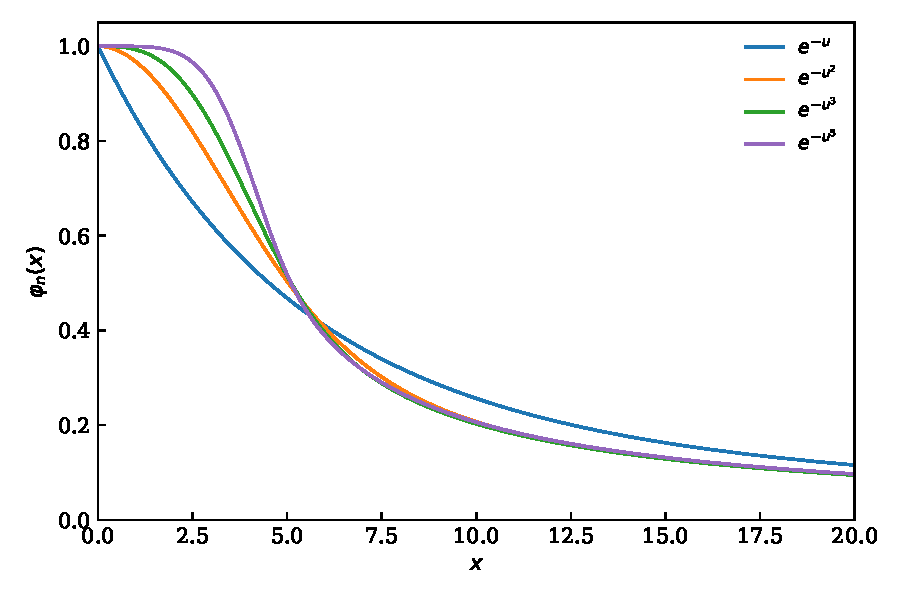
\includegraphics[width=0.78\textwidth]{fig_predictions_phi.pdf}
\caption{Master functions $\varphi_n(x)$ for the cutoff
family $f(u) = e^{-u^n}$.  All share $\varphi_n(0) = 1$
(the cutoff-independent IR limit) but differ at $x > 0$.
The exponential cutoff ($n = 1$) decays most slowly; sharper
cutoffs ($n \geq 2$) produce steeper descent and converge
toward a common profile.}
\label{fig:phi}
\end{figure}

% ============================================================
\section{Cutoff-dependent predictions}
\label{sec:fragile}
% ============================================================

The predictions in this section depend on the full shape of the
cutoff function~$f$ through the master
function~$\varphi_n(x)$~\eqref{eq:phi-n}.  They are
\emph{not} uniquely predicted without an additional principle
fixing~$f$.

\subsection{The cutoff function constraint}
\label{sec:constraint}

The requirement that the form factors $F_1$, $F_2$ be entire
functions of $z = \Box/\Lambda^2$ restricts the class of
admissible cutoff functions.  For the family
$f(u) = e^{-u^\alpha}$, entireness holds if and only if
$\alpha \in \mathbb{N}$ (positive integer).  At non-integer
$\alpha$ (e.g., $\alpha = 3/2$), the function $u^\alpha$ has a
branch point at $u = 0$, and the resulting form factors inherit
branch cuts.  Power-law cutoffs $f(u) = (1 + u)^{-N}$ are
likewise excluded.

The conventional choice $f(u) = e^{-u}$ ($n = 1$) is
computationally convenient but not uniquely determined.  The
choices $e^{-u^2}$, $e^{-u^3}$, etc., are equally admissible.

\subsection{Cutoff function scan}
\label{sec:bands}

To illustrate the sensitivity of cutoff-dependent predictions to
the choice of~$f$, we compute the propagator zeros by formally
substituting $\varphi \to \varphi_n$ in the form
factors~\eqref{eq:hC-scalar}--\eqref{eq:hC-vector}.  This
substitution is evaluated at finite~$z$ (the propagator zeros
lie at $z_0 > 2$, far from the $z \to 0$ divergence that arises
for $n \geq 2$; see Section~\ref{sec:formfactors}).
Table~\ref{tab:bands} reports the results for
$n \in \{1, \ldots, 5\}$.

\begin{table}[ht]
\centering
\caption{Cutoff function scan for $f(u) = e^{-u^n}$.  Here $z_0$
is the first positive real zero of $\Pi_{\mathrm{TT}}(z)$,
obtained by formal substitution $\varphi \to \varphi_n$
in~\eqref{eq:hC-scalar}--\eqref{eq:hC-vector}, and $V(1)/V_N$
is the modified Newtonian potential at $r\Lambda = 1$.  For
all~$n$, $\alpha_C(0) = 13/120$ (cutoff-independent).  The
zeros $z_0$ are computed at finite~$z$ where the formal
substitution is well-defined; the $z \to 0$ limit diverges for
$n \geq 2$ (see text).  This family does not exhaust all
admissible cutoff functions; wider families could produce values
outside the shown range.}
\label{tab:bands}
\begin{tabular}{ccccc}
\toprule
$n$ & $x \cdot \varphi_n(x \to \infty)$
& $z_0$ & $m_2/\Lambda$ & $V(1)/V_N$ \\
\midrule
1 & $2.00$ & $2.415$ & $1.554$ & $0.718$ \\
2 & $1.77$ & $5.174$ & $2.274$ & $0.863$ \\
3 & $1.79$ & $5.248$ & $2.291$ & $0.865$ \\
4 & $1.81$ & $5.229$ & $2.287$ & $0.865$ \\
5 & $1.84$ & $5.208$ & $2.282$ & $0.864$ \\
\bottomrule
\end{tabular}
\end{table}

For $n \geq 2$, the fakeon mass lies in the range
$m_2/\Lambda \in [2.274, 2.291]$ (spread~$0.7\%$).  The $n = 1$
(exponential) cutoff is an outlier at $m_2/\Lambda = 1.554$;
the exponential form factor changes sign at a lower value of~$z$
than the sharper ($n \geq 2$) cutoffs, pulling the propagator
zero closer to the origin.

The Stelle Lagrangian mass
$m_{\mathrm{Stelle}} = \Lambda\sqrt{60/13} \approx 2.148\,
\Lambda$ (from the local approximation
$\Pi_{\mathrm{TT}} \approx 1 + c_2 z$) differs from all five
pole masses in Table~\ref{tab:bands} because the nonlocal form
factor modifies the zero position.

\begin{figure}[ht]
\centering
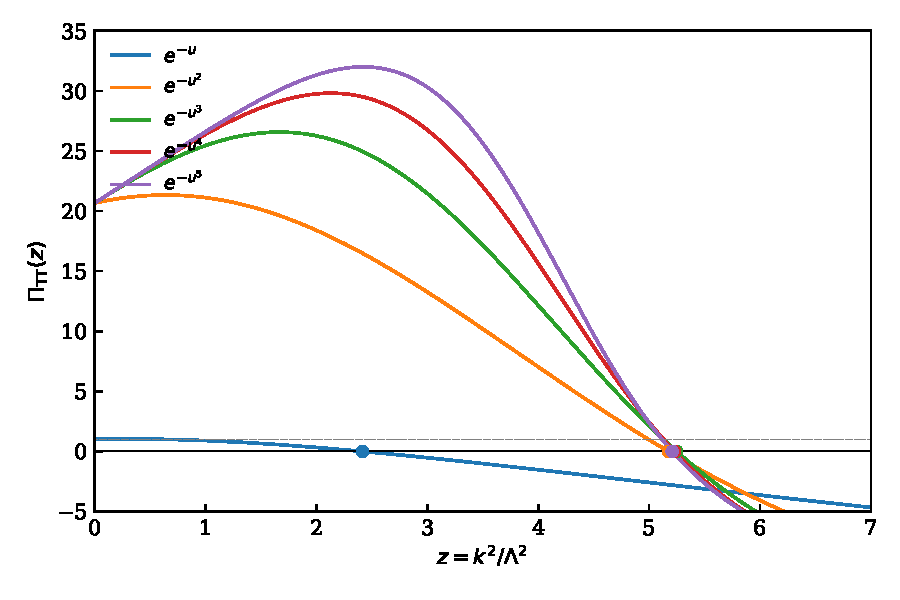
\includegraphics[width=0.78\textwidth]{fig_predictions_PiTT.pdf}
\caption{The dressed propagator denominator
$\Pi_{\mathrm{TT}}(z)$ for five cutoff functions.  Circles
mark the first positive real zero~$z_0$ (the fakeon pole).
The exponential cutoff ($n = 1$) crosses zero at
$z_0 = 2.41$; the sharper cutoffs ($n \geq 2$) cross near
$z_0 \approx 5.2$.}
\label{fig:PiTT}
\end{figure}

\subsection{Modified Newtonian potential}
\label{sec:potential}

At $\xi = 1/6$ (scalar mode absent), the modified Newtonian
potential takes the single-Yukawa form.  In the static limit,
the Fourier transform of the propagator~\eqref{eq:inv-prop}
gives $V(r) \propto \int \dd^3 k\, e^{i\mathbf{k}\cdot\mathbf{r}}
/ [k^2 \Pi_{\mathrm{TT}}(k^2/\Lambda^2)]$.  The residue of the
spin-2 pole at $\Pi_{\mathrm{TT}}(z_0) = 0$ is
$R_0 = 1/[z_0 \Pi'_{\mathrm{TT}}(z_0)] < 0$ (negative, since
$\Pi_{\mathrm{TT}}$ crosses zero from above).  The coefficient
$-4/3$ arises from the weight of the $P^{(2)}$ projector in the
tensor structure of the inverse propagator~\eqref{eq:inv-prop}:
\begin{equation}\label{eq:potential}
  \frac{V(r)}{V_N(r)} = 1 - \frac{4}{3}\,e^{-m_2 r},
\end{equation}
where $m_2 = \sqrt{z_0}\,\Lambda$ is the fakeon mass from
Table~\ref{tab:bands}.  In the Yukawa approximation,
$V(0)/V_N = -1/3$ (repulsive at the origin).  This is an
artifact of the local approximation: the full nonlocal potential,
defined by the Fourier integral of $1/\Pi_{\mathrm{TT}} - 1$,
diverges as $r \to 0$, since
$1/\Pi_{\mathrm{TT}} - 1 \to -1$ as $z \to \infty$.  The Yukawa
approximation is valid for $r \gg 1/\Lambda$.

At solar system distances ($r \sim 1\;\mathrm{AU}$), with
$\Lambda > 3.53\;\mathrm{meV}$.  This bound is obtained as
follows: at $\xi = 1/6$ the scalar mode is absent
(Section~\ref{sec:scalar}), and the
potential~\eqref{eq:potential} has a single Yukawa term with the
nonlocal mass $m_2 = 1.554\,\Lambda$~\eqref{eq:z0}.  The
E\"ot-Wash experiment~\cite{Kapner:2007} constrains the Yukawa
correction $|\alpha|\,e^{-r/\lambda}$ at
$\lambda = 1/m_2 = 1/(1.554\,\Lambda)$ and $|\alpha| = 4/3$,
giving $\Lambda > 3.53\;\mathrm{meV}$ (update of the
bound~\cite{Alfyorov:2026paper2}, previously obtained in the
two-component Stelle parametrization):
$m_2 r \sim 10^8$ and
$V/V_N = 1 - (4/3)\,e^{-10^8} = 1$ to exponential precision.

\begin{figure}[ht]
\centering
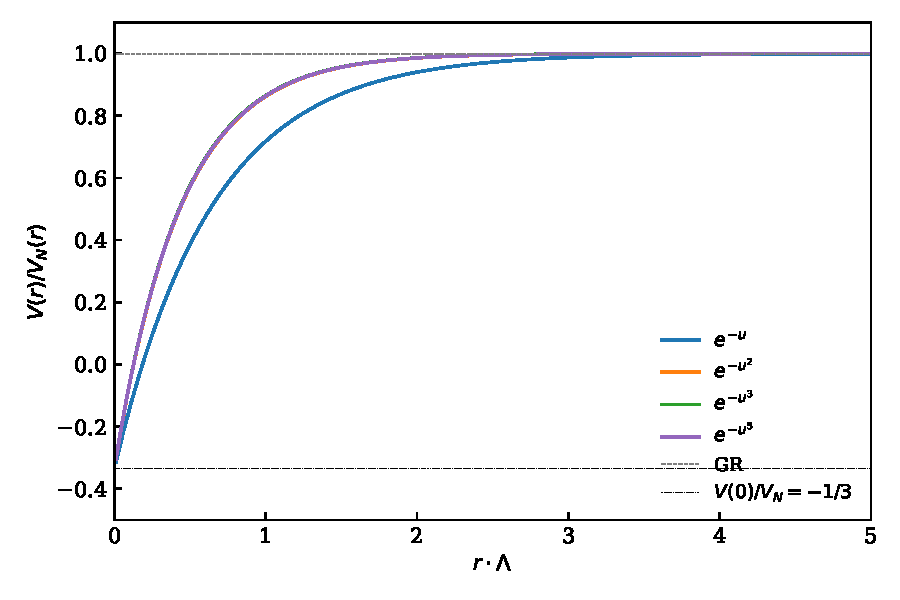
\includegraphics[width=0.78\textwidth]{fig_predictions_potential.pdf}
\caption{Modified Newtonian potential $V(r)/V_N(r)$ at
$\xi = 1/6$ for three cutoff functions ($n = 1, 2, 5$)
and the GR limit.  All cutoffs give $V(0)/V_N = -1/3$
(repulsive origin).  The spread narrows for $n \geq 2$.}
\label{fig:potential}
\end{figure}

\subsection{Graviton dispersion relation}
\label{sec:dispersion}

The linearized equation of motion for tensor perturbations is
$\Pi_{\mathrm{TT}}(\Box/\Lambda^2)\,\Box\, h_{\mu\nu} = 0$,
which in momentum space becomes
$\Pi_{\mathrm{TT}}(z)\cdot z = 0$ with
$z = (-\omega^2 + k^2)/\Lambda^2$.  This factors into two
branches:
\begin{enumerate}[(i)]
\item $z = 0$, i.e., $\omega^2 = k^2$: the massless graviton
  with $v_{\mathrm{ph}} = v_g = c$.  This mode is unmodified
  because $\Pi_{\mathrm{TT}}$ is a scalar multiplicative factor
  acting on the Lorentz-invariant combination~$k^2$.
\item $\Pi_{\mathrm{TT}}(z_0) = 0$: massive fakeon modes.
  These do not propagate as physical particles under the fakeon
  prescription.
\end{enumerate}

The massless graviton dispersion relation ($z = 0$ branch) is
$\omega^2 = k^2$ exactly at one loop: there is no
birefringence, and the signal velocity equals~$c$.  This is a
result about free propagation on flat background; on curved
backgrounds (e.g., Schwarzschild), the perturbation equation
acquires corrections $\sim c_2(\omega/\Lambda)^2$ from the
nonlocal form factor --- see Section~\ref{sec:qnm}.  Both
statements (Euclidean derivation) are conditional on the
correctness of the Wick rotation for form factors $F_1$ that
are entire functions of the complex argument.

This is compatible with the GW170817
bound~\cite{GW170817:2017}
$|c_T - c|/c < 10^{-15}$,
which SCT satisfies exactly (not approximately) at one loop.

% ============================================================
\section{What SCT does not predict}
\label{sec:negative}
% ============================================================

\subsection{No cosmological constant prediction}
\label{sec:cc}

The cosmological constant $\Lambda_{\mathrm{cc}}$ enters the
spectral action through the $a_0$ coefficient and the moment
$f_4 = \int_0^\infty f(u)\, u\, \dd u$ (in the Chamseddine--Connes
convention where $a_0 \propto f_4\, \Lambda^4$).  The physical
value of $\Lambda_{\mathrm{cc}}$ is not predicted; it is a free
parameter set by the choice of~$f_4$ and the
renormalization-group trajectory.  The spectral action
generically produces $a_0 \propto f_4 \Lambda^4$, which exceeds
the observed $\Lambda_{\mathrm{cc}} \sim 10^{-122}\, M_P^4$ by
${\sim}\,120$ orders of magnitude; SCT inherits the
cosmological constant problem from quantum field theory.  This
gap is shared by LQG, AS, and IDG.

\subsection{Black hole quasinormal modes}
\label{sec:qnm}

QNM frequency shifts in SCT receive two independent contributions:
\begin{enumerate}
\item \emph{Metric modification} (Level~2, computed):
  $\delta\omega/\omega \sim \exp(-m_2 r_{\mathrm{peak}})$.
  For GW150914 ($M = 62\,M_\odot$): $m_2 r_{\mathrm{peak}} = 7.78 \times 10^9$,
  giving $\log_{10}(\delta\omega/\omega) \approx -3.4 \times 10^9$.
\item \emph{Perturbation-equation correction} (parametric estimate):
  $\delta\omega/\omega \sim \order(1) \cdot c_2(\omega/\Lambda)^2$,
  where $c_2 = 13/60$ and $\order(1)$ is an unknown dimensionless
  coefficient depending on the open problem Gap~G1 (computation of
  $\delta\Theta^{(C)}_{\mu\nu}$ on the Schwarzschild background).
  For GW150914: $\omega/\Lambda \approx 3.4 \times 10^{-10}$, giving
  $\delta\omega/\omega \sim 10^{-20}$ up to the $\order(1)$ factor.
\end{enumerate}
Contribution~(2) dominates by $\sim 10^{3 \times 10^9}$ orders of magnitude.
Both are $\geq 15$ orders below LIGO sensitivity ($\sim 10^{-1}$).
Results for observed black holes are given in Table~\ref{tab:qnm}.
Numerical values are computed in the Stelle approximation
($m_2^{\mathrm{Stelle}} = \Lambda\sqrt{60/13} \approx 2.148\,\Lambda$);
for the exact propagator zero~\eqref{eq:z0}
($m_2 = 1.554\,\Lambda$ at $n=1$) the values of
$m_2 r_{\mathrm{peak}}$ decrease by $1.554/2.148 \approx 0.72$,
shifting $\log_{10}(\delta\omega/\omega)$ by $\sim 0.14$ ---
within the order-of-magnitude accuracy of the estimate.
At $\xi = 1/6$ the scalar mode decouples and
$h(r) = 1 - (4/3)\,e^{-m_2 r}$; the table is given for
$\xi = 0$ (both Yukawa modes) for generality.

\begin{table}[h]
\centering
\caption{SCT QNM frequency shifts for observed black holes ($l=2$, $n=0$).}
\label{tab:qnm}
\begin{tabular}{lccc}
\toprule
Object & $M/M_\odot$ & $m_2 r_{\mathrm{peak}}$ &
  $\log_{10}(\delta\omega/\omega)_{\mathrm{total}}$ \\
\midrule
$10\,M_\odot$  & 10    & $1.3 \times 10^9$  & $-17.9$ \\
GW150914       & 62    & $7.8 \times 10^9$  & $-19.5$ \\
GW190521       & 142   & $1.8 \times 10^{10}$ & $-20.3$ \\
Sgr\,A*        & $4.15 \times 10^6$ & $5.2 \times 10^{14}$ & $-29.2$ \\
M87*           & $6.5 \times 10^9$ & $8.2 \times 10^{17}$ & $-35.5$ \\
\bottomrule
\end{tabular}
\end{table}

\begin{figure}[t]
\centering
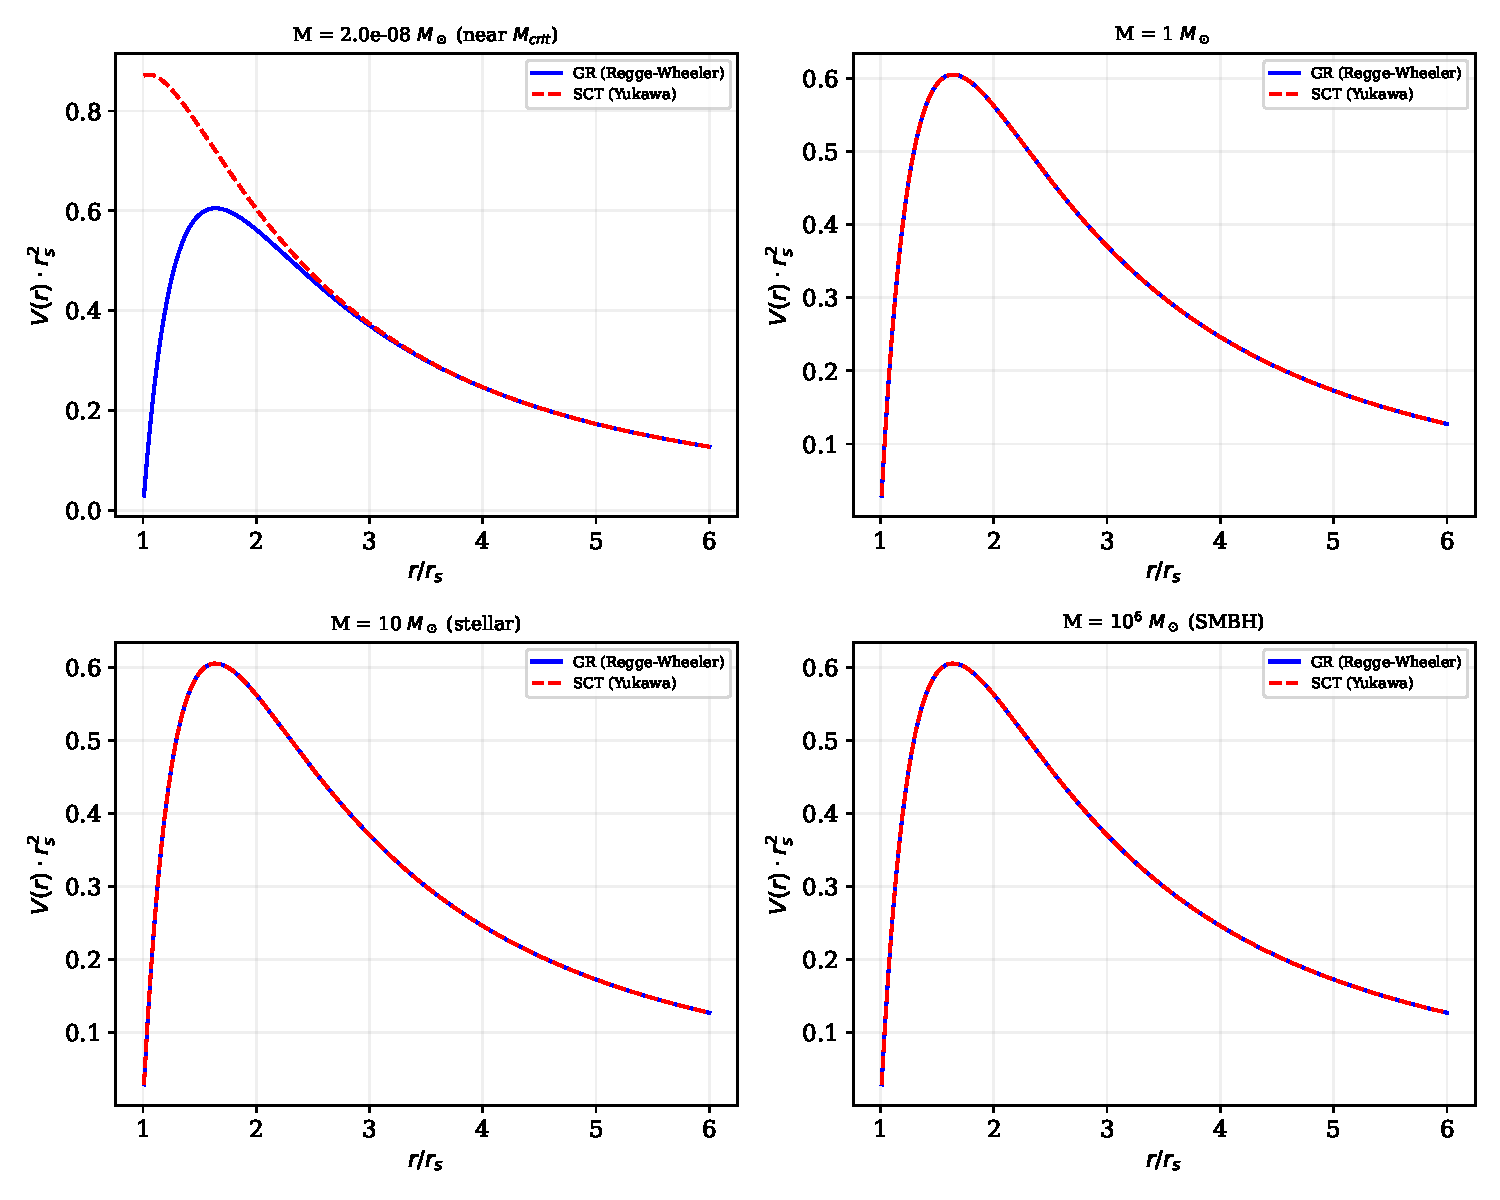
\includegraphics[width=\textwidth]{fig_qnm_potentials.pdf}
\caption{Regge--Wheeler potentials ($l=2$): GR (blue) vs.\ SCT (red dashed)
at four masses. Top left: near $M_{\mathrm{crit}}$, modification is $O(1)$.
Other panels: modification is exponentially suppressed and invisible.}
\label{fig:qnm_potentials}
\end{figure}

\paragraph{Quantum corrections dominate classical ones.}
The one-loop quantum correction to QNM frequencies is
$\delta\omega_{\mathrm{quantum}}/\omega \sim (l_P/r_s)^2 c_{\log}
\sim 10^{-78}$ for $10\,M_\odot$ ($c_{\log} = 37/24$).
The classical SCT metric correction:
$\delta\omega_{\mathrm{SCT}}/\omega \sim e^{-10^9} \ll 10^{-78}$.
Quantum corrections dominate by $\sim 10^{10^9 - 78}$ orders.
The exponential suppression of the classical correction is
independently confirmed in local quadratic gravity by
Antoniou, Gualtieri and Pani~\cite{Antoniou:2025,Antoniou:2026}.

\paragraph{Mode stability.}
For odd (axial) parity, an analytic theorem holds: the full
Regge--Wheeler potential
$V_{\mathrm{odd}}^{\mathrm{SCT}} = (f/r^2)[\ell(\ell+1) - 3(1-f) + r_s h'(r)]$
satisfies $V > 3f/r^2 > 0$ for all $r > r_H$, $\ell \geq 2$,
using $h' > 0$ and $0 < f < 1$ outside the horizon.
By the Kay--Wald theorem~\cite{KayWald:1987} this excludes growing modes.

\paragraph{Tidal Love numbers.}
In GR, $k_2 = 0$ exactly for black holes~\cite{BinningtonPoisson:2009}.
In SCT, $k_2 \neq 0$ (qualitative difference from GR), but
$|k_2| \sim \exp(-m_2 r_s)$: unmeasurable for astrophysical objects.

\paragraph{Gravitational echoes.}
The SCT potential has exactly \emph{one} external maximum for all
$M > M_{\min}$. No cavity (double-barrier) structure forms;
gravitational echoes are structurally impossible.

\paragraph{Superradiance.}
For astrophysical BHs: $\alpha = m_2 M \gg 1$, no quasi-bound
states.  The boundary $\alpha = 1$ at
$m_2 = 1.554\,\Lambda$ and $\Lambda = 3.53\;\mathrm{meV}$ gives
$M_{\alpha=1} = 1/(m_2 G) \approx 5 \times 10^{-8}\,M_\odot$;
the lower bound $M_{\min} \approx 1.4 \times 10^{-8}\,M_\odot$
is the minimum mass for which a horizon
exists~\cite{Alfyorov:2026paper2}.  In the window
$M_{\min} < M < M_{\alpha=1}$, a horizon exists with $\alpha < 1$;
without the fakeon prescription, a standard ghost would trigger
superradiant instability.  The fakeon projects out on-shell states
and prevents cloud formation.

\paragraph{Kerr and Reissner--Nordstr\"om.}
For Kerr at $a/M = 0.998$, the dominant correction rises to
$\sim 10^{-17}$ (from $\sim 10^{-20}$ at $a = 0$), still unmeasurable.
For extremal Reissner--Nordstr\"om ($Q/M \to 1$): $\sim 10^{-18}$.

\paragraph{QNM bounds on $\Lambda$.}
In the Cardoso et al.\ parametrization~\cite{Cardoso:2019},
the Yukawa correction maps to $\alpha_j = 0$ for all $j$
(beyond-all-orders in $r_H/r$). The formal LIGO ringdown bound:
$\Lambda_{\mathrm{QNM}} \sim 2.2 \times 10^{-12}\;\mathrm{eV}$,
nine orders weaker than $\Lambda_{\mathrm{E\ddot{o}t\text{-}Wash}} > 3.53\;\mathrm{meV}$.

\begin{figure}[t]
\centering
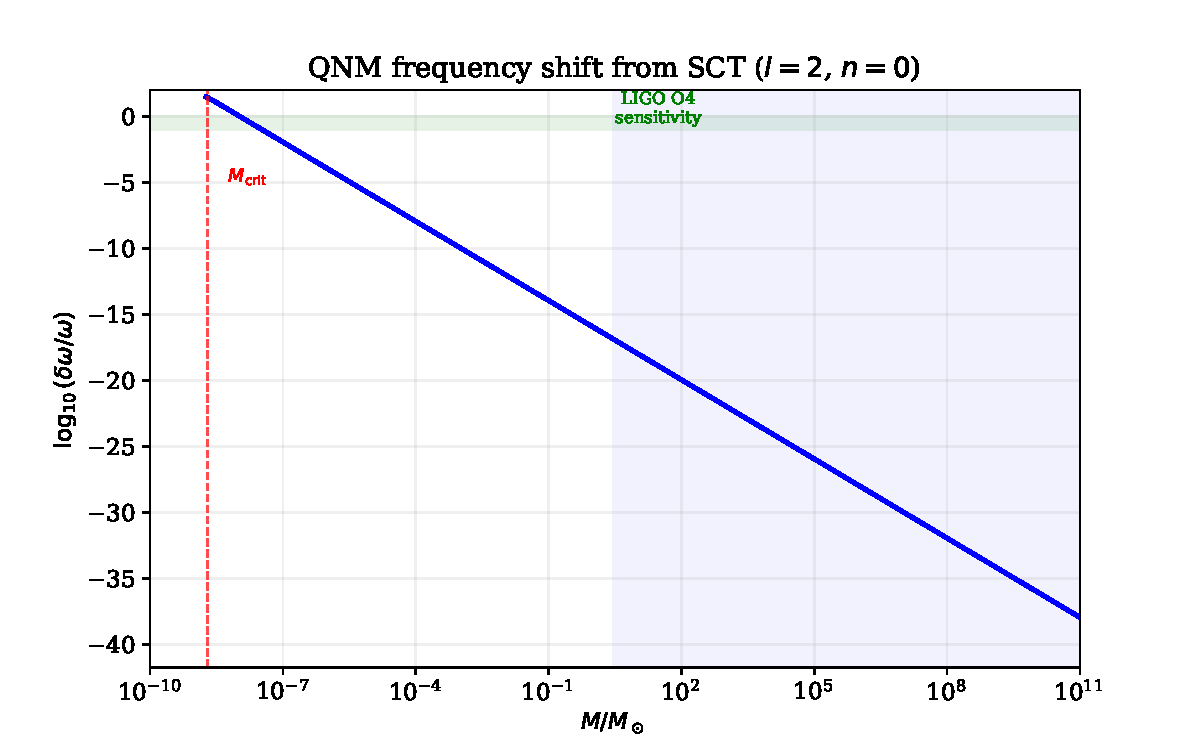
\includegraphics[width=\textwidth]{fig_qnm_mass_scan.pdf}
\caption{Total QNM frequency shift $\delta\omega/\omega$ vs.\ BH mass
($l=2$, $n=0$). For small masses ($M \lesssim M_{\min}$): metric
modification $\sim e^{-m_2 r_{\mathrm{peak}}}$ dominates. For
astrophysical masses ($M \gtrsim 1\,M_\odot$): perturbation-equation
correction $\sim c_2(\omega/\Lambda)^2$ dominates. Green band: LIGO
O4 sensitivity.}
\label{fig:qnm_mass_scan}
\end{figure}

\paragraph{Summary of $\Lambda$ bounds.}
Different channels span 21 orders of magnitude (Table~\ref{tab:lambda_bounds}).

\begin{table}[h]
\centering
\caption{Bounds on the cutoff scale $\Lambda$ from different channels.}
\label{tab:lambda_bounds}
\begin{tabular}{lll}
\toprule
Channel & $\Lambda_{\min}$ & Source \\
\midrule
GW dispersion (GWTC-3) & $> 8.50\;\mathrm{meV}$ & \cite{GWTC3} \\
\textbf{E\"ot-Wash (dedicated)} & $\boldsymbol{> 3.53\;\mathrm{meV}}$ & this work \\
E\"ot-Wash (Stelle) & $> 2.57\;\mathrm{meV}$ & \cite{Alfyorov:2026paper2}, superseded \\
Solar system (Cassini) & $> 2.38\;\mathrm{meV}$ & \cite{Alfyorov:2026paper2}, superseded \\
LIGO ringdown (QNM) & $> 2.2 \times 10^{-12}\;\mathrm{eV}$ & this work \\
BH shadow (EHT) & $\sim 10^{-30}\;\mathrm{eV}$ & this work \\
\bottomrule
\end{tabular}
\end{table}

\subsection{Other null predictions}
\label{sec:astro_other}

Beyond QNMs, the following observables are indistinguishable from GR:
\begin{itemize}
\item Neutron star structure (unmodified TOV equation),
\item Late-time cosmology ($\delta H^2/H^2 \sim 10^{-64}$;
  \cite{Alfyorov:2026paper4}).
\end{itemize}

\subsection{Swampland tension}
\label{sec:swampland}

The SCT scalaron potential (if the scalaron existed) would
violate the refined de~Sitter Swampland
conjecture~\cite{Obied:2018} at $\order(1)$ parameter values.
The curvature condition has a hard ceiling
$\eta_{\min} = -1/3$, which cannot satisfy the Swampland
parameter $\tilde{c} \sim 1$.

Since $\xi = 1/6$ eliminates the scalaron entirely, this
tension is moot for the standard spectral action: there is no
scalar potential to test against the conjecture.  Confirmation
of pure Starobinsky inflation by CMB-S4 or
LiteBIRD~\cite{LiteBIRD:2022} would increase the tension
between the Swampland programme and $R^2$-type models in
general.

% ============================================================
\section{Comparison with competing programs}
\label{sec:comparison}
% ============================================================

\subsection{Programs compared}
\label{sec:programs}

We compare SCT with five quantum gravity programs:
\emph{Loop Quantum Gravity}
(LQG)~\cite{Rovelli:2004,Thiemann:2007}, based on
non-perturbative canonical quantization with spin-network
states;
\emph{Asymptotic Safety}
(AS)~\cite{ReuterSaueressig:2012}, based on the existence of a
non-Gaussian UV fixed point of the gravitational RG flow;
\emph{Causal Dynamical Triangulations}
(CDT)~\cite{AJL:2012}, a lattice approach with a causal
constraint on the path integral;
\emph{string theory}~\cite{Polchinski:1998}, based on
one-dimensional extended objects replacing point particles; and
\emph{Infinite Derivative Gravity}
(IDG)~\cite{BMS:2006,Modesto:2012}, which modifies the graviton
propagator with an entire-function form factor to achieve
ghost-freedom.
We do not include Causal Set Theory~\cite{BLMS:1987} as a
separate entry: it does not by itself produce the quantitative
predictions listed in the comparison axes, though
the CJ bridge formula~\cite{Alfyorov:2026paper7} connects
SCT to causal-set observables.

\subsection{Comparison table}
\label{sec:table}

Table~\ref{tab:comparison} presents the comparison across nine
quantitative axes.  Each cell contains the best available
numerical value (or status assessment) from the primary
literature.

\begin{table}[ht]
\centering
\caption{Cross-program comparison.  Abbreviations: n.c.\ = not
computed, m.d.\ = model-dependent, n.p.\ = not predicted.
References are given in the text.}
\label{tab:comparison}
\small
\begin{tabular}{p{2cm}p{1.7cm}p{1.7cm}p{1.7cm}p{1.4cm}p{1.7cm}p{1.7cm}}
\toprule
Axis & SCT & LQG & AS & CDT & String & IDG \\
\midrule
$d_S$(UV)${}^a$ &
  method-dep. &
  ${\sim}\,2$ &
  $2$ (exact) &
  $1.80\pm0.25$ &
  m.d. &
  $2$ \\[4pt]
$c_{\log}$ &
  $+37/24$ &
  $-1/2$ &
  $0$ or $\pi/g_*$ &
  n.c. &
  charge-dep. &
  no log \\[4pt]
Singularity &
  unresolved${}^b$ &
  bounce &
  $G \to 0$ &
  n.c. &
  fuzzball &
  resolved \\[4pt]
$n_s$, $r$ &
  excluded &
  $r = 0.07$--$0.17$~\cite{AguloMorris:2015} &
  $r \approx 0.003$ &
  n.c. &
  landscape &
  $n_s = 1{-}2/N$ \\[4pt]
Dispersion &
  $\omega = k$${}^c$ &
  m.d. &
  n.c. &
  n.c. &
  unmod. &
  unmod. \\[4pt]
$\gamma_{\text{PPN}}$ &
  $1$ &
  $1$ &
  $1$ &
  n.c. &
  $1$ &
  $1$ \\[4pt]
UV prop. &
  entire${}^d$ &
  spinfoam &
  power-law &
  lattice &
  string-scale &
  Gaussian \\[4pt]
$\Lambda_{\text{cc}}$ &
  n.p. &
  n.p. &
  n.p. &
  $>0$ req. &
  $10^{500}$ &
  n.p. \\[4pt]
Matter &
  $\alpha_C = 13/120$ &
  free &
  FP bounds &
  n.c. &
  landscape &
  minimal \\
\bottomrule
\end{tabular}

\smallskip\noindent{\footnotesize
${}^a$ SCT value depends on definition.  In the Mittag-Leffler
method, $d_S$ passes through ${\approx}\,2$ near the ghost scale,
but the flow is non-monotonic (oscillatory), unlike the monotonic
$4 \to 2$ transition in CDT/AS/LQG.  Under the HK definition:
$d_S = 4$; ASZ: $d_S = 0$.

\noindent ${}^b$ Yukawa potential gives $V(0)/V_N = -1/3$; the
full nonlocal potential diverges as $r \to 0$ (one loop).

\noindent ${}^c$ One-loop result.

\noindent ${}^d$ Entire function of order~1; the fakeon prescription
for countably many complex poles requires a convergence proof.}
\end{table}

\begin{figure}[ht]
\centering
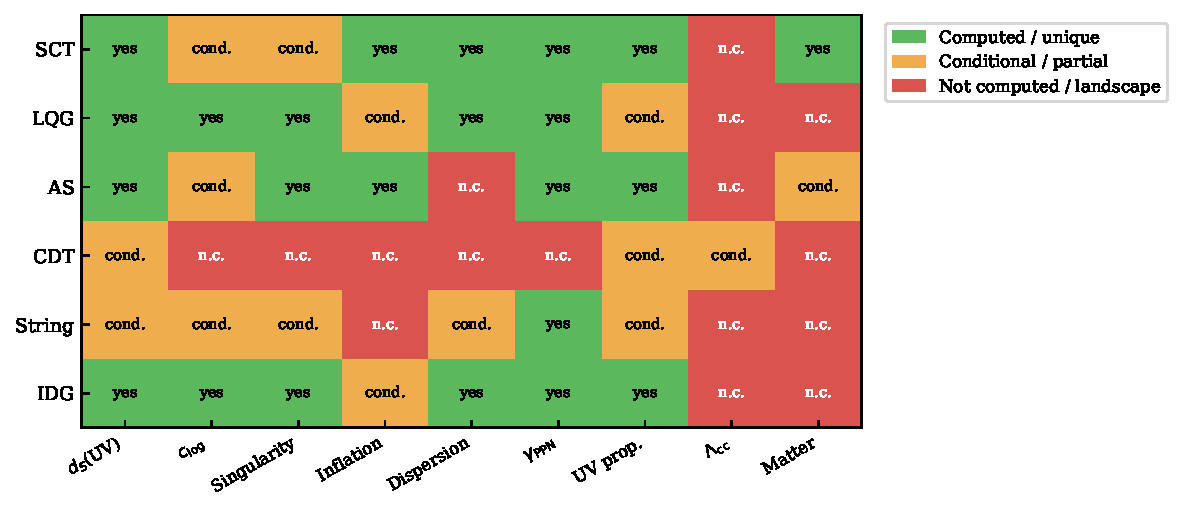
\includegraphics[width=0.95\textwidth]{fig_predictions_heatmap.pdf}
\caption{Prediction status across six quantum gravity programs
and nine axes.  Green: computed or unique prediction.  Yellow:
conditional or partial.  Red: not computed or
landscape-dependent.  SCT has computed entries on 8/9~axes;
CDT has computed entries on 2/9.}
\label{fig:heatmap}
\end{figure}

\subsection{Discriminating observables}
\label{sec:discriminating}

Three axes yield predictions that are mutually incompatible
across programs:
\begin{enumerate}[(1)]
\item \textbf{$c_{\log}$.} SCT: $+37/24$. LQG: $-1/2$.
  Opposite sign.  AS: definition-dependent.  IDG: no logarithmic
  correction.  A measurement of $c_{\log}$ (e.g., through black
  hole area quantization signatures in LISA
  data~\cite{LISA:2023}) would sharply discriminate between
  programs.

\item \textbf{UV propagator.}  SCT: entire function of order~1.
  IDG: Gaussian $e^{-k^2/M^2}/k^2$.  AS: power-law
  $G(k) \to g_*/k^2$.  LQG: discrete spinfoam amplitude.  These
  are four qualitatively distinct analytic structures.

\item \textbf{Matter coupling.}  SCT: $\alpha_C = 13/120$,
  determined by the SM particle content alone.  AS: the
  non-Gaussian fixed point constrains the number of matter
  fields but does not fix the coupling coefficient.  LQG,
  string, IDG: matter coupling is a free input.  SCT is the
  only program in this comparison where the zero-momentum
  gravitational coupling coefficient $\alpha_C(0) = 13/120$
  is determined by the SM particle content alone, without
  additional free parameters.
\end{enumerate}

\subsection{SCT and asymptotic safety}
\label{sec:AS}

SCT and AS share identical matter one-loop form factors: the
Codello--Zanusso basis function
$f_C(x) = 1/(12x) + (\varphi - 1)/(2x^2)$~\cite{CZ:2012}
coincides with $h_C^{(0)}(x)$~\eqref{eq:hC-scalar}.  This
identity holds for any cutoff function (it is a property of the
heat kernel, not of the RG scheme).

The first divergence occurs at the graviton loop level.
Including graviton and ghost contributions, the full one-loop
AS Weyl coefficient
is~\cite{SCM:2010}
\begin{equation}\label{eq:AS-alphaC}
  \alpha_C^{\mathrm{AS}} = \frac{13}{120} + \frac{7}{20}
  = \frac{11}{24} \approx 0.458
  = 4.23\;\alpha_C^{\mathrm{SCT}}.
\end{equation}
The comparison~\eqref{eq:AS-alphaC} does \emph{not} compare
like with like: $\alpha_C^{\mathrm{SCT}}$ sums only over matter
loops (the spectral action is a trace over matter fields),
whereas $\alpha_C^{\mathrm{AS}}$ includes also graviton and
Faddeev--Popov ghost contributions.  The agreement of the matter
part ($13/120$) is a nontrivial cross-check, not a prediction
of a new effect.  These graviton-loop contributions are absent in
the SCT spectral action (which sums over matter fields only).

The UV universality classes differ: SCT form factors are entire
functions (the propagator saturates at a finite constant in the
deep UV), while AS predicts power-law running with anomalous
dimension $\eta_N = -2$ at the fixed
point~\cite{KRS:2022}.

\subsection{Universal features}
\label{sec:universal}

The spectral dimension $d_S \to 2$ in the UV is obtained by
SCT, LQG, AS, and IDG.  CDT gives $d_S = 1.80 \pm 0.25$
(original measurement
by~\cite{AJL:2005}, within $1\sigma$ of~2).  This
near-universality across disparate approaches has been noted
by~\cite{Carlip:2017}.

All six programs predict $\gamma_{\mathrm{PPN}} = 1$ at solar
system scales.  No program predicts a specific value for the
cosmological constant.

% ============================================================
\section{Falsification criteria}
\label{sec:falsification}
% ============================================================

Table~\ref{tab:falsification} lists observations that would
contradict specific SCT predictions.

\begin{table}[ht]
\centering
\caption{Falsification criteria.  Each row states an observation
that would contradict the indicated SCT prediction, the
experiment that could make the observation, and the approximate
timeline.}
\label{tab:falsification}
\begin{tabular}{p{3.2cm}p{3.5cm}p{2.5cm}c}
\toprule
Observation & Implication for SCT & Experiment & Timeline \\
\midrule
Scalar GW polarization detected &
  $\xi \neq 1/6$; standard spectral triple insufficient &
  ET/CE network & 2035+ \\[4pt]
$c_{\log} < 0$ &
  App.~\ref{app:clog} derivation wrong; LQG prediction favored &
  theoretical${}^e$ & --- \\[4pt]
GW birefringence detected &
  Parity violation in gravity; discrete structure (LQG-type) &
  Fermi-LAT, CTA & ongoing \\[4pt]
Short-range deviation at $r > 56\;\mu$m &
  $\Lambda < 3.53\;\mathrm{meV}$; phenomenology requires
  revision &
  Torsion balance & 2030s \\[4pt]
$r \approx 0.003$ from $R^2$ inflation &
  $\alpha_R \neq 0$, hence $\xi \neq 1/6$ or BSM &
  CMB-S4, LiteBIRD & 2028--32 \\
\bottomrule
\end{tabular}

\smallskip\noindent{\footnotesize
${}^e$The criterion is theoretical: $c_{\log}$ is falsified by an
independent computation of the sign in a competing program, not
by direct experimental measurement (for astrophysical BHs,
$\ln(A/\ell_P^2) \sim 10^2$, which is unmeasurable at current
precision).}
\end{table}

We emphasize that detection of a scalar GW polarization would
not falsify SCT as a framework, but would require replacing the
standard spectral triple with a BSM extension in which
$\xi \neq 1/6$.

% ============================================================
\section{Discussion}
\label{sec:discussion}
% ============================================================

SCT is a one-loop gravitational effective field
theory~\cite{Donoghue:1994}, valid through two loops under the
$D^2$-quantization chirality
theorem~\cite{Alfyorov:2026paper3}.  At three loops, the
existence of three independent quartic Weyl invariants versus one
spectral-function parameter creates a structural
overdetermination~\cite{Alfyorov:2026paper3}.  The theory is
therefore best characterized as an EFT valid through $L = 2$,
not as a UV-complete quantum gravity theory.

The cutoff function $f$ introduces an infinite-dimensional
ambiguity in the form factors, but the predictions testable at
macroscopic scales with current technology (PPN parameters, GW
speed, absence of scalar mode) all lie in the cutoff-independent
sector.  We note that while the ratio $\alpha_C = 13/120$ is
$f$-independent, the absolute magnitude of the $C^2$ term
in the action involves the moment $f_4 = \int_0^\infty
f(u)\, u\, \dd u$, which depends on~$f$.  The
cutoff-dependent predictions (effective masses, potential shape,
spectral dimension flow) are bounded but not uniquely
determined.  Off-shell quantities (propagator zeros, effective
masses) are additionally gauge-dependent; the on-shell
predictions (scattering amplitudes, PPN parameters) are
gauge-invariant.

The spectral action~\eqref{eq:spec-action} is formulated in
Euclidean signature.  The continuation to Lorentzian signature
follows Barvinsky and Vilkovisky~\cite{BV:1990} via Wick
rotation of the form factor arguments; the fakeon
prescription~\cite{Anselmi:2017} operates in Lorentzian
signature.  A fully non-perturbative Lorentzian formulation of
the spectral action remains an open problem.

The fakeon prescription resolves the unitarity problem at one
loop.  The extension to all orders requires proving that
Anselmi's finite-threshold argument~\cite{Anselmi:2018}
generalizes to the countably infinite pole set of the SCT
propagator.  This remains an open problem.

Among the six programs compared, SCT is the only one where the
matter coupling coefficient $\alpha_C$ is fully determined by
the Standard Model particle content.  This is a consequence of
the spectral action principle, which derives the gravitational
effective action from the spectrum of the Dirac operator coupled
to matter.

% ============================================================
\section{Conclusions}
\label{sec:conclusions}
% ============================================================

We have cataloged the predictions of Spectral Causal Theory and
classified them by their dependence on the cutoff function~$f$.
The results are:

\begin{enumerate}[(1)]
\item Two unconditional predictions: $\alpha_C = 13/120$ and
  $c_1/c_2 = -1/3$ at $\xi = 1/6$
  (Table~\ref{tab:robust}).  Two established: absence of the
  scalar mode at $\xi = 1/6$ and exclusion of Starobinsky
  inflation.  Three conditional: PPN parameters and $c_T = c$
  (conditional on the generalized fakeon prescription and Wick
  rotation) and $c_{\log} > 0$ (conditional on the Sen formula
  and field content; value $37/24$ for SM, $8/5$ for
  SM$+\nu_R$).

\item Cutoff-dependent predictions
  (Table~\ref{tab:bands}): the fakeon mass
  $m_2/\Lambda = 1.554$ at $n = 1$ (rigorously justified
  cutoff); results for $n \geq 2$ are formal extrapolations
  (see the caveat in the table).

\item The massless graviton ($z = 0$) has dispersion
  $\omega = k$ at one-loop level (Euclidean derivation), with
  no birefringence.  QNM corrections on curved backgrounds are
  $\sim \order(1) \cdot c_2(\omega/\Lambda)^2$ --- a parametric
  estimate with an unknown $\order(1)$ factor (Gap~G1 open).

\item Three discriminating observables: the \emph{sign} of
  $c_{\log}$ (not the value), UV propagator analytic structure,
  and matter coupling coefficient.

\item Five falsification criteria stated
  (Table~\ref{tab:falsification}).

\item Within the fakeon prescription, SCT is consistent with all
  current observational data.  Modifications to GR are suppressed
  at macroscopic scales:
  power-law ($\sim \order(1) \cdot c_2(\omega/\Lambda)^2
  \sim 10^{-20}$ up to the $\order(1)$ factor for the
  perturbation-equation correction) and exponentially
  ($\sim e^{-m_2 r_s}$ for the metric modification).

\item Modal stability of SCT-Schwarzschild proven analytically
  for odd parity ($V > 3f/r^2 > 0$, $\ell \geq 2$).  Tidal
  Love numbers $k_2 \neq 0$ (qualitative GR difference),
  gravitational echoes structurally impossible (single-barrier
  potential), superradiant instability prevented by the fakeon
  prescription (Table~\ref{tab:qnm}).
\end{enumerate}

The strongest discriminant between SCT and competing programs is
the \emph{sign} of the logarithmic black hole entropy correction:
$c_{\log} > 0$ (SCT, for any field content with the dominant
graviton contribution) versus $c_{\log} < 0$ (LQG, $-1/2$ or
$-3/2$ depending on the method).

% ============================================================
\appendix
\section{Cutoff function scan}
\label{app:cutoff}
% ============================================================

The generalized master function for $f(u) = e^{-u^n}$ is
\begin{equation}\label{eq:phi-n-app}
  \varphi_n(x) = \int_0^1
  \exp\bigl(-[\alpha(1-\alpha)\, x]^n\bigr)\, \dd\alpha.
\end{equation}
At $x = 0$: $\varphi_n(0) = 1$ for all~$n$ (the integrand
reduces to~$1$).  For $n = 1$: $\varphi_1'(0) = -1/6$.  For
$n \geq 2$: $\varphi_n'(0) = 0$ because the chain rule produces
a factor $x^{n-1}$ that vanishes at $x = 0$.  The leading
correction is then set by the $n$-th derivative:
$\varphi_n(x) = 1 + \order(x^n)$.

The first positive real zero~$z_0$ of
$\Pi_{\mathrm{TT}}(z)$ was located using Brent's method
(SciPy~\texttt{brentq}) after a sign-change scan over
$z \in [0.1, 20]$ with step size~$0.05$.  All computations
used 50-digit arithmetic (mpmath).  The $n = 1$ result
$z_0 = 2.4148$ was cross-checked against the canonical SCT
codebase~\cite{Alfyorov:2026repo}, with agreement to all
50~digits.

% ============================================================
\section{Derivation of $c_{\log} = 37/24$}
\label{app:clog}
% ============================================================

The one-loop logarithmic correction to the Bekenstein--Hawking
entropy for a non-extremal Schwarzschild black hole is given by
the Sen formula~\cite{Sen:2012}:
\begin{equation}\label{eq:sen-formula}
  c_{\log} = \frac{1}{180}\bigl[
  2\,N_s + 7\,N_F - 26\,N_V + 424\bigr],
\end{equation}
where $N_s$ is the number of real scalars, $N_F$ the number of
Dirac fermions, $N_V$ the number of gauge vectors, and
$+424$ is the graviton contribution~\cite{Sen:2012}.
Sen's convention uses $\ln a_H$ where $A_H \sim a_H^2$; our
$c_{\log}$ is the coefficient of $\ln(A_H/\ell_P^2)$, hence the
prefactor $1/180 = 1/(2 \times 90)$.  The
coefficient $-26$ per vector arises from the proper vector
determinant ($+62$) minus two Faddeev--Popov ghosts
($2 \times 44 = 88$), giving $62 - 88 = -26$.  The fermion
coefficient is $+7$ per Dirac fermion (not $+7/2$ per Weyl).
The formula uses zeta-function regularisation on the Euclidean
Schwarzschild instanton with Dirichlet boundary conditions at
the horizon.

For the Standard Model field content ($N_s = 4$,
$N_F = 22.5$, $N_V = 12$):
\begin{center}
\begin{tabular}{lrc}
\toprule
Field & Coefficient & Contribution \\
\midrule
Scalars  & $2 \times 4$ & $+8$ \\
Fermions & $7 \times 22.5$ & $+157.5$ \\
Vectors  & $-26 \times 12$ & $-312$ \\
Graviton & & $+424$ \\
\midrule
Total    & & $277.5$ \\
\bottomrule
\end{tabular}
\end{center}
Therefore
\begin{equation}\label{eq:clog-result}
  \boxed{c_{\log} = \frac{277.5}{180}
  = \frac{37}{24} \approx 1.542\,.}
\end{equation}
The matter contribution alone is $-146.5/180 < 0$ (dominated by
vector Faddeev--Popov ghosts); the graviton term $+424$ makes the
total positive.

\begin{remark}[Cross-checks]
Pure gravity ($N_s = N_F = N_V = 0$):
$c_{\log}^{\mathrm{pure}} = 424/180 = 106/45 \approx 2.36$,
consistent with Sen's $C_{\mathrm{local}} = 212/45$ after the
$\ln a_H \to \ln A_H$ conversion~\cite{Sen:2012}.  The computation has been verified
by exact rational arithmetic ($\mathrm{Fraction}(555,2)/180
= \mathrm{Fraction}(37,24)$) and agrees with the conformal
anomaly approach using the coefficients $a = 1/360$,
$c = 1/120$ per real scalar~\cite{BirDav:1982}.

This gives the local heat-kernel contribution; ensemble-dependent
zero-mode corrections (Sen~\cite{Sen:2012}, Section~4.2:
$\delta c_{\log} \in [-3/4,\, 0]$) shift $c_{\log}$ by at most
$-3/4$ without changing its sign.  The sign of $c_{\log}$ is
positive for the SM,
opposite to the LQG prediction
($c_{\log}^{\mathrm{LQG}} = -1/2$
or $-3/2$~\cite{Meissner:2004,KaulMajumdar:2000}).
\end{remark}

% ============================================================
\section*{Acknowledgments}
% ============================================================

We thank Igor Shnyukov for collaboration on
``Weyl curvature from the Hasse diagram''~\cite{Alfyorov:2026paper7}.

\section*{Data availability}

All numerical data, computational scripts, and verification
results are available in the SCT Theory
repository~\cite{Alfyorov:2026repo}.  The comparison table
data are stored in machine-readable JSON format.

\section*{Declarations}

\subsection*{Conflict of interest}
The author declares no conflict of interest.

\subsection*{Use of AI tools}
Large language models (Claude, Anthropic) were used for code generation
and numerical verification scripting. All mathematical derivations,
physical arguments, and scientific conclusions were formulated and
verified by the author. The AI-generated code was independently
validated against analytical results at 100-digit precision.

\bibliographystyle{unsrtnat}
\bibliography{../references/sct_predictions}

\end{document}
